\section{پیشنیازها}
حالا کمی به پیشنیازهای هندسه دیفرانسیل(هندسه خمینه‌ها یا منیفلدها) و هندسه ریمانی(منیفلدهایی که به تانسور متریک مجهز هستند) می‌پردازیم. اولین چیز تعریف خود منیفلد است. شاید تعریف دقیق ریاضی و مجرد آن خیلی برای هدف ما لازم نباشد, با این وجود اشاره کوتاهی به آن می‌کنیم.
\subsection{منیفلد چیست؟}
در این بخش تعریف منیفلد را میاوریم و روی خاصیت‌هایی از آن که برای درک کلی مفهوم واجب هستند تاکید بیشتری می‌کنیم.
\begin{figure}[h!]
    \centering
    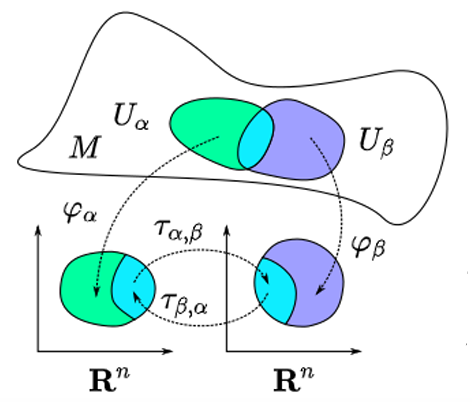
\includegraphics[width=0.4\textwidth]{Pictures/Q2/1.png}
    \caption{تصویر شماتیک از یک منیفلد با دو تا از چارت‌هایش}
\end{figure}\\
منیفلد یک فضای توپولوژیک مجهز به یک توپولوژی هاسدورف است که توسط تعدادی مجموعه باز(اعضای توپولوژی) پوشانده می‌شود که به این مجموعه‌های باز که منیفلد را می‌پوشانند چارت گفته می‌شود. هر کدام از این چارت‌ها با زیرمجموعه بازی از $\mathbb{R}^N$ (که در اینجا به $N$ بعد منیفلد گفته می‌شود) همسان ریخت(Homeomorphic) است. در اشتراک بین چارت‌ها باید دیفیومورفیزم(Diffeomorphism) بین آنها برقرار باشد.\\
\\
این تعریف به صورت شهودی به این معنی است که منیفلد موجودی است که به صورت موضعی با تعداد ثابتی مختصه که اعداد حقیقی هستند توصیف می‌شود. در نواحی‌ای که چارت‌ها با هم اشتراک دارند باید تبدیل از یک مختصات به مختصات دیگر به صورت وارون پذیر, پیوسته و مشتق‌پذیر انجام شود. با رعایت کردن این جزییات متوجه ایرادهایی که در قسمت قبل از مختصات قطبی گرفتیم می‌شویم. برای مثال اگر منیفلد را یک حلقه یا $S^1$ در نظر بگیریم متوجه می‌شویم که اگر این حلقه را با یک چارت بخواهیم بپوشانیم دچار مشکل می‌شویم چون که یا به یک نقطه بیش از یک مختصه نسبت می‌دهیم یا ناپیوستگی ایجاد می‌کنیم. و برای پوشاندن این حلقه به دست کم دو چارت نیاز داریم.\\
\\
در عمل برای هندسه اطلاعات این موضوع که به بیشتر از یک چارت برای پوشاندن منیفلد نیاز داشته باشیم کم پیش میاید و در اکثر مواقع می‌توانیم فرض کنیم که برای منیفلدهایی که ما با آن‌ها کار می‌کنیم می‌توانیم کل آن را با یک چارت بپوشانیم.
\pagebreak

\subsection{چگونه بردار و ‌هم‌بردار تعریف کنیم؟}
موجود ریاضی دیگری که باید تعریف کنیم بردارها و هم‌بردارها هستند. برای اینکار میتوانیم به صورت شهودی تصور کنیم که منیفلد در یک فضای $\mathbb{R}^M$ که در آن $M$ بزرگتر از بعد منیفلد است نشانده(Embede) شده است. حالا ما برای تعریف بردار میتوانیم بردارهای مماس بر هر نقطه منیفلد را در نظر بگیریم. یعنی به عبارتی در هر نقطه از منیفلد یک فضای برداری جداگانه تعریف کنیم که شامل بردارهای مماس از فضای بزرگتر در آن نقطه است.
\begin{figure}[h!]
    \centering
    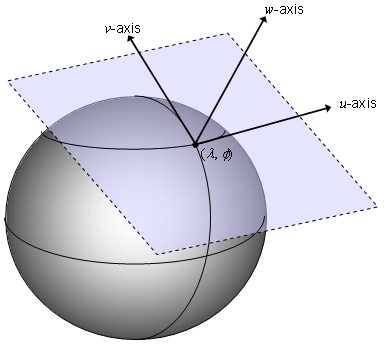
\includegraphics[width=0.4\textwidth]{Pictures/Q2/2.jpg}    
    \caption{تعریف شهودی فضای مماس}
\end{figure}\\
اما برای این موضوع نیز تعریف دقیق تری وجود دارد که بدون نشاندن منیفلد در فضای بزرگتر ممکن است و به جهاتی بسیار کاربردی‌تر هم هست. به دو روش بردارها یا فضای مماس را تعریف می‌کنند. این دو روش با هم معادل‌اند.\\
\\
روش اول: در نظر گرفتن خم‌هایی که از نقطه مدنظر منیفلد عبور می‌کنند. آن دسته از خم‌هایی که پس از اعمال نگاشت نقشه(نگاشت از منیفلد به فضای پارامترها) شیب یکسانی در فضای پارامترها دارند را در نظر میگیریم. به کلاس هم‌ارزی این خم‌ها می‌گوییم یک بردار. برای اینکه این موجودهای ساخته شده واقعا فضای برداری تشکیل دهند باید جمع بردارها و ضرب عدد در بردار را تعریف کنیم. یک تعریف طبیعی برای این عمل‌ها می‌توان انجام این عمل‌ها روی شیب‌ها در فضای پارامترها باشد. سپس باید نشان دهیم که این جمع بردارها و ضرب عدد در بردار که تعریف کرده‌ایم خوش تعریف است یعنی به انتخاب نماینده از کلاس هم‌ارزی بستگی ندارد. پس از آن باید اثبات کنیم که این اعمال تعریف شده خواص فضای برداری را برقرار می‌کنند. چک کردن این امرها کار ساده‌ای است که به راحتی می‌توان انجام داد.\\
\\
روش دوم: تعریف بردارها به صورت عملگرهای دیفرانسیلی مرتبه اول که روی توابع مشتق پذیر از منیفلد به اعداد حقیقی اثر می‌کنند. منظور از مرتبه اول بودن این است که علاوه بر خطی بودن باید خاصیت لایبنیتزی داشته باشند. یعنی اگر منیفلد $\mathcal{M}$ را داشته باشیم داریم:
\begin{equation}
    f,g:\mathcal M\longrightarrow\mathbb{R},\quad a,b\in \mathbb{R},\quad X\in T_P\mathcal{M},
\end{equation}
\begin{equation}
    \Longrightarrow X(a\ f+b\ g)=a\ X(f)+b\ X(g),\quad X(fg)=X(f)g(P)+f(P)X(g)
\end{equation}\\
این تعریف در اکثر مواقع کاربردی تر است. همچنین فضای دوگان که آن را با $T_P^*\mathcal{M}$ نشان می‌دهیم به صورت فضای دوگان $T_P\mathcal{M}$ تعریف می‌شود.\\
\begin{figure}[h!]
    \centering
    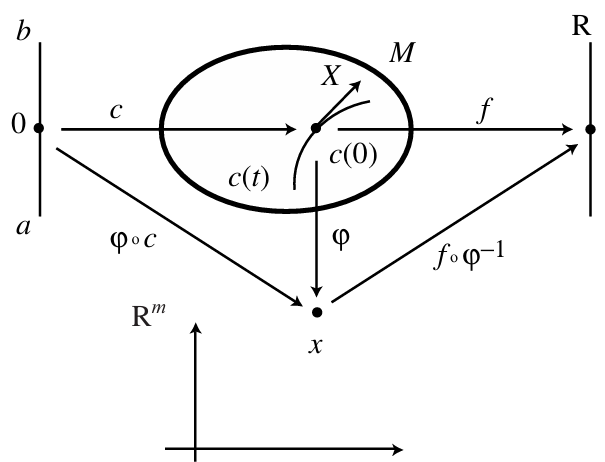
\includegraphics[width=0.4\textwidth]{Pictures/Q2/3.png}
    \caption{تعریف اول از بردارها}
\end{figure}\\
همچنین می‌توانیم میدان‌های برداری و هم‌برداری تعریف کنیم. برای میدان‌های برداری که آن‌ها را با $\mathfrak{X}$ نشان می‌دهیم دقیقا مانند خود بردارها تعریف می‌شوند با این تفاوت که به ازای هر نقطه یک بردار داریم بنابراین باید در این دو خاصیت صدق کند:
\begin{equation}
    f,g:\mathcal M\longrightarrow\mathbb{R},\quad a,b\in \mathbb{R},\quad X\in \mathfrak{X},
\end{equation}
\begin{equation}
    \Longrightarrow X(a\ f+b\ g)=a\ X(f)+b\ X(g),\quad X(fg)=X(f)\ g+f\ X(g)
\end{equation}\\
میدان‌های هم‌برداری نیز به صورت مشابه با اثر کردن روی میدان‌های هم برداری و بدست آوردن یک میدان اسکالر تعریف می‌شوند.\\
\\
حالا که فضاهای برداری و هم‌برداری را تعریف کردیم می‌توانیم با ضرب تانسوری آن‌ها فضاهای حاصل ضربی را نیز بسازیم:
$$T_P^*\mathcal{M}\otimes T_P\mathcal{M}\otimes T_P \mathcal{M} \otimes T_P^* \mathcal{M} \otimes T_P\mathcal{M}\otimes\dots$$
همچنین برای میدان‌های تانسوری به صورت مشابه می‌توانیم عمل کنیم.\\
\\
\subsection{هندسه ریمانی}
حالا با معرفی تانسور متریک, سرفصل جدیدی از هندسه به نام هندسه ریمانی را معرفی می‌کنیم. تانسور متریک تعریف ضرب داخلی بردارها است. به این معنی که ضرب داخلی دو بردار $X,Y\in T_P\mathcal{M}$ را با صورت زیر تعریف میکنیم:
\begin{equation}
    \langle X,Y\rangle :=g(X,Y)
\end{equation}
که در آن $g\in T_P^*\mathcal{M}\otimes T_P^*\mathcal{M}$ تانسور متریک است. از آنجایی که این تانسور نشان دهنده ضرب داخلی است یک تانسور متقارن است و اگر به صور ت ماتریسی به آن نگاه کنیم یک ماتریس مثبت معین است. از تانسور متریک می‌توان برای تعریف فاصله بین نقاط نزدیک به هم استفاده کرد طوری که اگر دو نقطه اختلاف مختصه‌هایشان به صورت $d\theta^i$ باشد آن وقت فاصله آن دو نقطه به توان دو به صورت زیر می‌باشد:
\begin{equation}
    ds^2=g_{ij}d\theta^id\theta^j
\end{equation}
که در اینجا از نمادگذاری جمع انیشتین استفاده شده یعنی روی اندیس‌های تکراری جمع زده می‌شود.\\
حالا که فضاهای ضرب تانسوری و میدان‌های تانسوری را معرفی کردیم می‌توانیم فرم‌های دیفرانسیلی را معرفی کنیم. فرم‌های دیفرانسیلی خود یک بحث بسیار مفصل در هندسه دیفرانسیل هست که توضیح آن‌ها در اینجا شاید خیلی مناسب نباشد. تنها چیزی که به آن نیز داریم تا در یکی از کاربردهای هندسه اطلاعات از آن استفاده کنیم فرم حجم ناوردا است که در اینجا رابطه‌اش را می‌آوریم:
\begin{equation}
    \omega=\sqrt{\det g}\ d\theta^1\wedge d\theta^2\wedge \dots \wedge d\theta^N
\end{equation}
این فرم دیفرانسیلی نقش عنصر حجم را هنگام انتگرال گیری روی منیفلد بازی می‌کند. ویژگی خاص آن این است که تحت تغییر مختصات ناوردا است. که این ویژگی از همان عبارت $\sqrt{\det g}$ بدست میاید. اگر بخواهیم به صورت خیلی ساده به آن فکر کنیم میتوانیم به تغییر متغیر عادی در انتگرال‌ها و دترمینان ژاکوبی فکر کنیم. عبارت رادیکال دترمینان متریک نقش یک بر روی دترمینان ژاکوبی را بازی میکند. برای همین است که این عنصر حجم ناوردا است.\\
\\
موضوع دیگری که در هندسه ریمانی مطرح می‌شود \lr{Affine Connection} و مشتق همورد(\lr{Covariant Derivative}) است. که یک جور تعمیم مشتق جهتدار است. البته تعمیم‌های دیگری نیز مانند مشتق لی وجود دارند که تفاوت‌های عمیقی با مشتق هموردا دارد. به صورت کلی مشتق هموردا را به صورت زیر نمایش می‌دهیم:
\begin{equation}
    \nabla_XY
\end{equation}
که مشتق نسبت به $Y$ است در جهت $X$ ویژگی های این مشتق به صورت زیر اند:
\begin{equation}
    \nabla_X(Y_1+Y_2)=\nabla_X Y_1+\nabla_X Y_2,\quad \nabla_X(fY)=X(f) Y+f\nabla_X Y
\end{equation}
\begin{equation}
    \nabla_{X_1+X_2}Y=\nabla_{X_1} Y+\nabla_{X_2} Y,\quad \nabla_{f X}Y=f \nabla_X Y
\end{equation}
از روی این مشتق دو مفهوم دیگر که اهمیت زیادی دارند ظاهر می‌شوند. مفاهیم منحنی‌های ژئودزی و انتقال موازی. به صورت خیلی ساده منحنی های ژئودزی تعمیم خط راست به فضاهای خمیده هستند. \lr{Optimal Transport} یکی از موضوع‌های مهمی است که از طریق مفهوم ژئودزی به هندسه اطلاعات ارتباط پیدا میکند. از آنجایی که منحنی های ژئودزی تحت شرایطی منحنی های با کمترین طول بین دو نقطه از منیفلد هستند. به صورت ساده اگر به ژئودزی فکر کنم می توانیم معادله حاکم بر آن را بدست بیاوری. از آنجایی که قرار است تعمیمی از خط راست باشد داریم:
\begin{equation}
    \nabla_{\dot{\gamma}(t)}\dot{\gamma}(t)\propto \dot{\gamma}(t)
\end{equation}
ضریب تناسب به پارامتر خم یعنی $t$ بستگی دارد. اگر پارامتر خم را متناسب با طول یا به اصطلاح پارامتر آفین انتخاب کنیم ضریب تناسب صفر می‌شود و داریم:
\begin{equation}
    \nabla_{\dot{\gamma}(t)}\dot{\gamma}(t)=0
\end{equation}
اگر معادله بالا را برحسب مولفه‌ها باز کنیم داریم:
\begin{equation}
    \ddot{\theta^i}+\Gamma^i_{\ jk}\dot{\theta}^i\dot{\theta}^j=0
\end{equation}
که در آن $\Gamma^i_{\ jk}$ ضرایب کریستوفل هستند که به صورت زیر تعریف می‌شوند:
\begin{equation}
    \Gamma^i_{\ jk}=d\theta^i(\nabla_{\partial_j}\partial_k)
\end{equation}
در اینجا و در قبل تر از نمادهای $\partial_i$ و $d\theta^i$ به ترتیب برای بردارهای پایه وابسته به مختصات و بردارهای پایه فضای دوگان وابسته به مختصات استفاده کرده‌ایم(البته این نمادگذاری گاهی باعث اشتباه می‌شود از آنجایی که بعضی اوقات به اختلاف کوچک در پارامترها نیز $d\theta^i$ نسبت می‌دهیم. مانند رابطه‌ای که برای فاصله نقاط نزدیک به هم نوشتیم$ds^2=g_{ij}d\theta^i d\theta^j$ در اینجا $d\theta^i$ به معنی هم‌بردار نیست.). در حالت کلی هر $\nabla$ ای که ویژگی‌های گفته شده را برقرار کند یک \lr{Affine Connection} معتبر است. اما یک \lr{Affine Connection} خاص که از روی متریک بدست میاید وجود دارد که به آن \lr{Levi-Civita Connection} گفته می‌شود. ویژگی آن این است که متریک را ثابت نگه میدارد و مشتق هموردای متریک طبق این کانکشن صفر می‌شود $\nabla_X g=0$, که به راحتی میتوان رابطه‌ای برای ضرایب کریستوفل این کانکشن بر حسب مشتقات متریک حساب کرد.\\
\\
موضوع دیگر انتقال موازی است. انتقال موازی یک بردار به معنی حرکت یک بردار اولیه از یک فضای مماس اولیه روی یک خمی از منیفلد به نقطه نهایی است طوری که تاجای ممکن بردار دست نخورد. این را میتوان اینطوری فرمول بندی کرد که مشتق هموردای بردار در راستای خم صفر باشد. ویژگی دیگر کانکشن لوی چویتا این است که اگر دو بردار را با این کانکشن انتقال موازی دهیم ضرب داخلی دوبردار نهایی با ضرب داخلی دو بردار اولیه برابر است. به عبارتی اگر انتقال موازی تحت خم $c(t)$ و کانکشن آفین $\prod^\nabla_{c(t)}$ نشان دهیم داریم:
\begin{equation}
    \left\langle \prod^\nabla_{c(t)} X, \prod^\nabla_{c(t)} Y\right\rangle=     \left\langle X,  Y\right\rangle
\end{equation}

\subsection{ساختارهای هندسی دوگان}
در قسمت قبل با کانکشن لوی چویتا آشنا شدیم که ضرب داخلی را تحت انتقال موازی حفظ میکرد. حالا اگر کانکشنی غیر از لوی چویتا داشته باشیم میتوانیم یکه کانکشن دیگر که مزدوج آن باشد به این صورت تعریف کنیم:
\begin{equation}
    \left\langle \prod^{\nabla^*}_{c(t)} X, \prod^\nabla_{c(t)} Y\right\rangle=     \left\langle X,  Y\right\rangle
\end{equation}
که در آن $\nabla^*$ کانکشن مزدوج با کانکشن اولیه $\nabla$ است. به راحتی می‌توان دید که اگر میانگین این دو کانکشن را در نظر بگیریم به همان کانکشن لوی چویتا میرسیم. این ساختار که کمی از اصل هندسه ریمانی فاصله دارد در هندسه اطلاعات بسار مفید واقع می‌شود.\\
تا اینجا صحبتی از انحنای منیفلد نکردیم. برای محاسبه انحنا نیاز به تعریف تانسور ریمان داریم که در اینجا نمی گنجد. از روی تانسور ریمان می‌توان معیار مختلف کوچکتری برای نشان دادن انحنا پیدا کرد. قضیه ای به نام قضیه اساسی هندسه اطلاعات وجود دارد که بیان می‌کند که اگر یک منیفلد طبق کانکشن $\nabla$ تخت یا بدون انحنا باشد طبق کانکشن مزدوج آن یعنی $\nabla^*$ نیز تخت خواهد بود. در واقع قضیه کلی تر از این است و بیان میکند که اگر انحنای ثابت $\alpha$ داشته باشیم آنگاه با کانکشن مزدوج نیز همان انحنای ثابت را در منیفلد داریم, اما ما با همان حالت تخت سر و کار خواهیم داشت چون که همانطور که جلوتر می‌بینیم برای دو خانواده مهم توزیع ها یعنی خانواده نمایی و میکسچر ها این ویژگی برقرار است.